\begin{figure}[t]
  \centering
  % 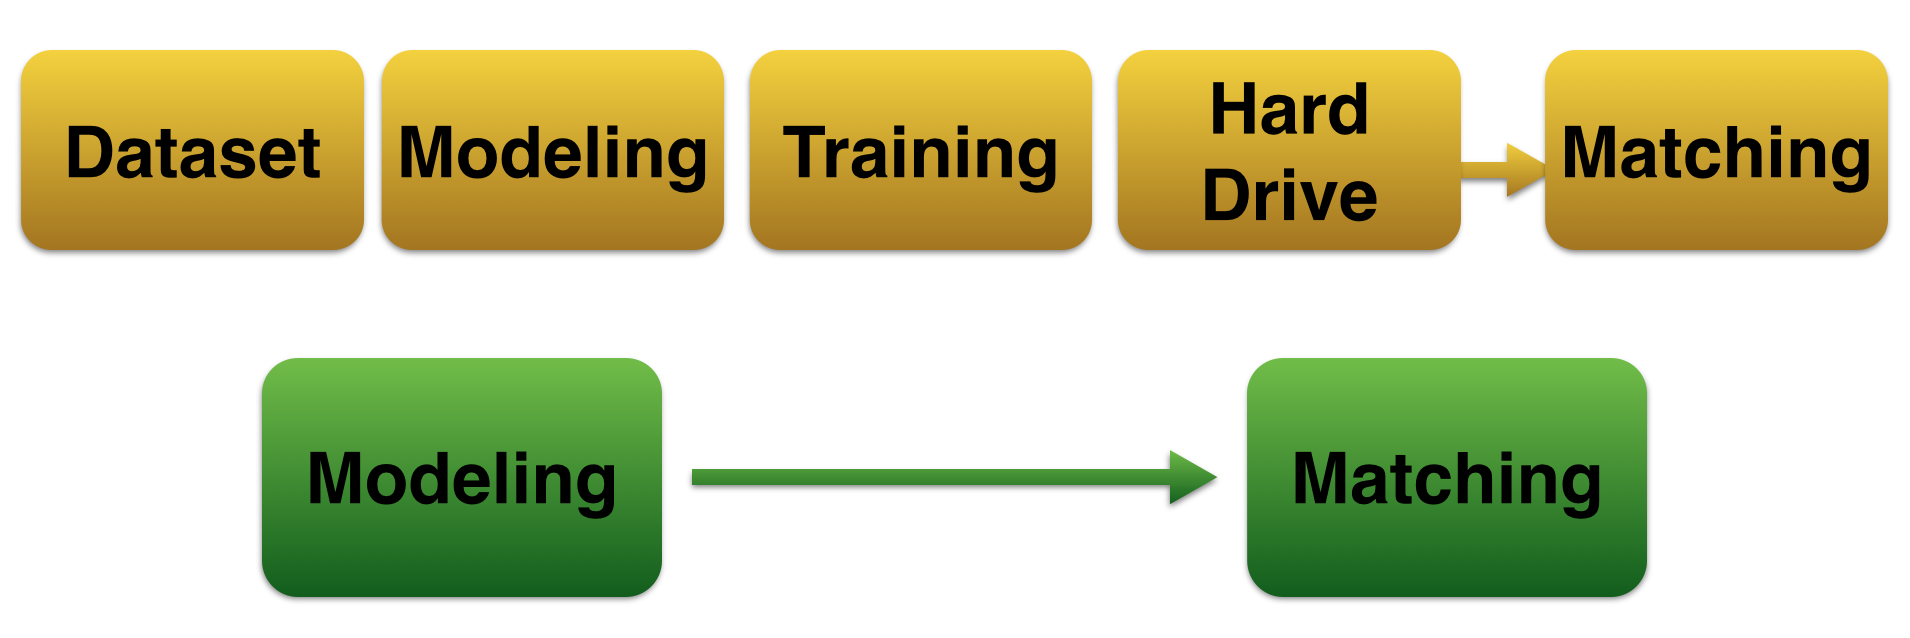
\includegraphics[width=0.9\linewidth]{schematics} 
  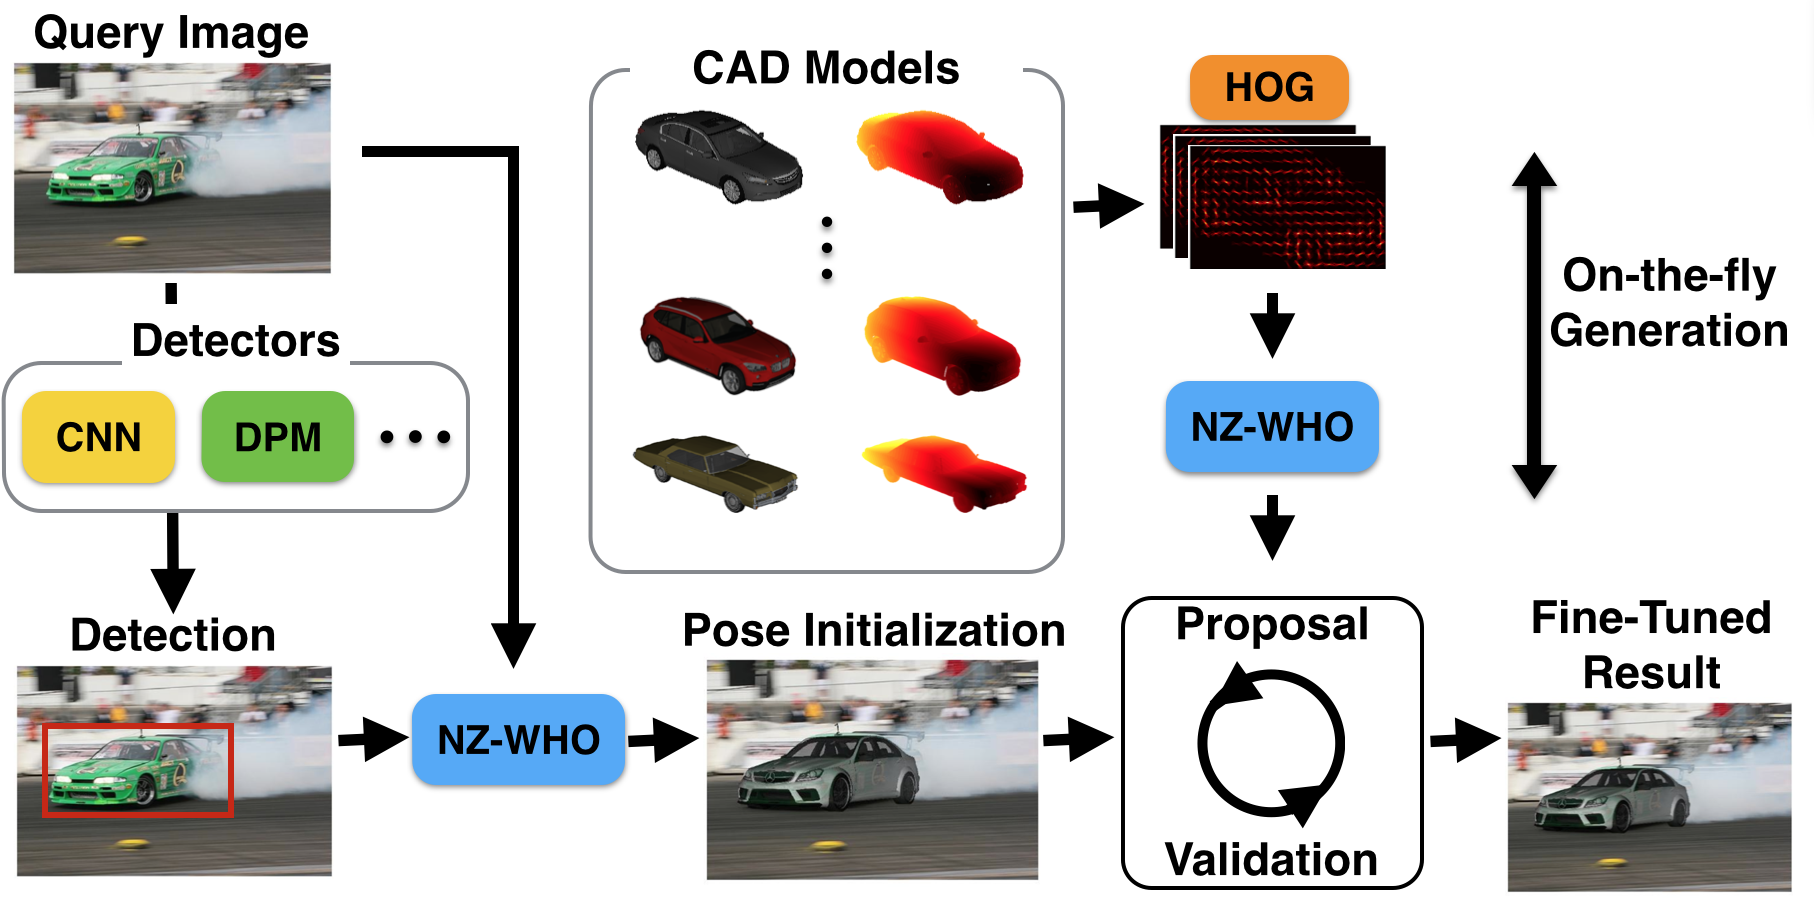
\includegraphics[width=0.99\linewidth]{front} % \\[-5pt]
  % (a)\\[0pt]
  % \setlength\tabcolsep{0pt}
  % \begin{tabular}{cc}
  %     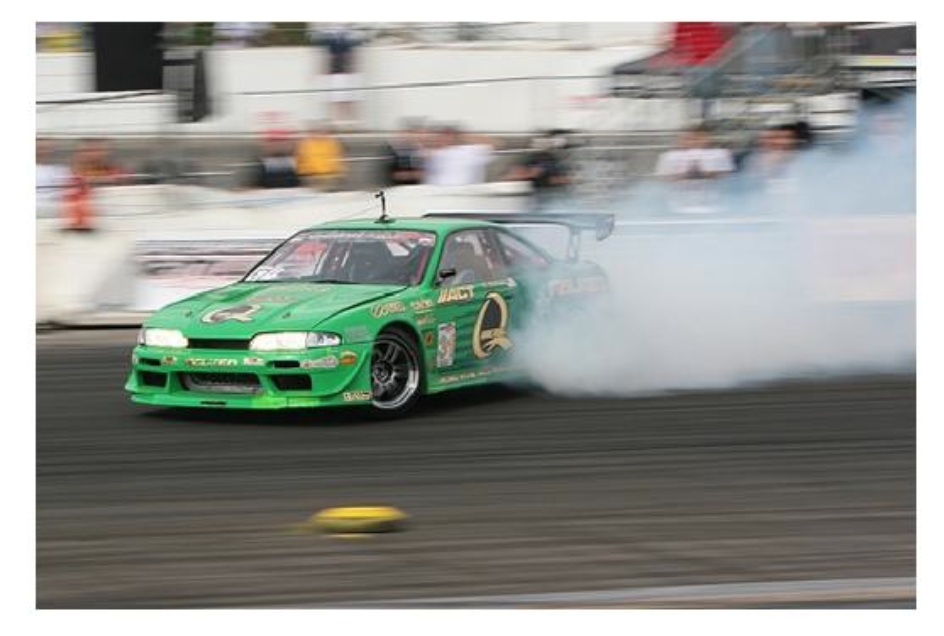
\includegraphics[width=0.45\linewidth]{car/orig2} & 
  %     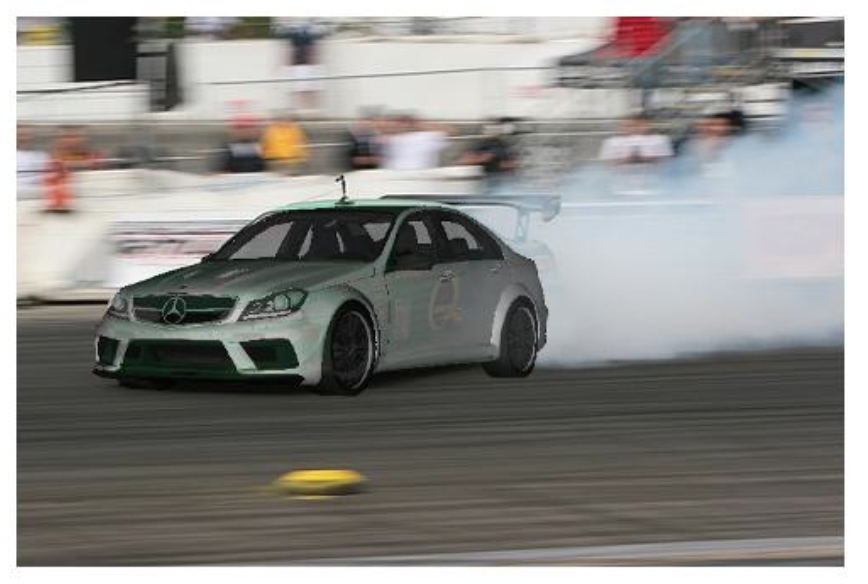
\includegraphics[width=0.45\linewidth]{car/overlay2}
  %  %   \begin{tabular}{cc}
  %  %       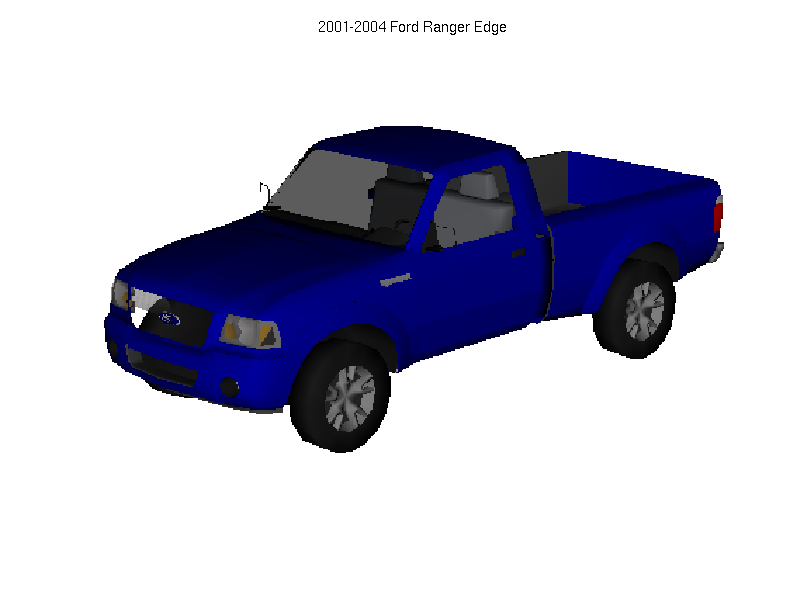
\includegraphics[width=0.16\linewidth]{cad_car/2001-2004 Ford Ranger Edge} & 
  %  %       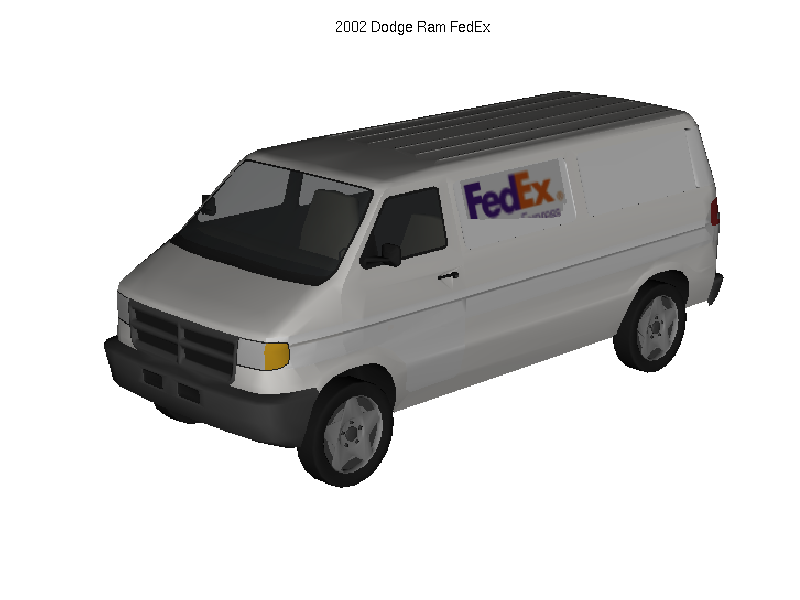
\includegraphics[width=0.16\linewidth]{cad_car/2002 Dodge Ram FedEx} \\ 
  %  %       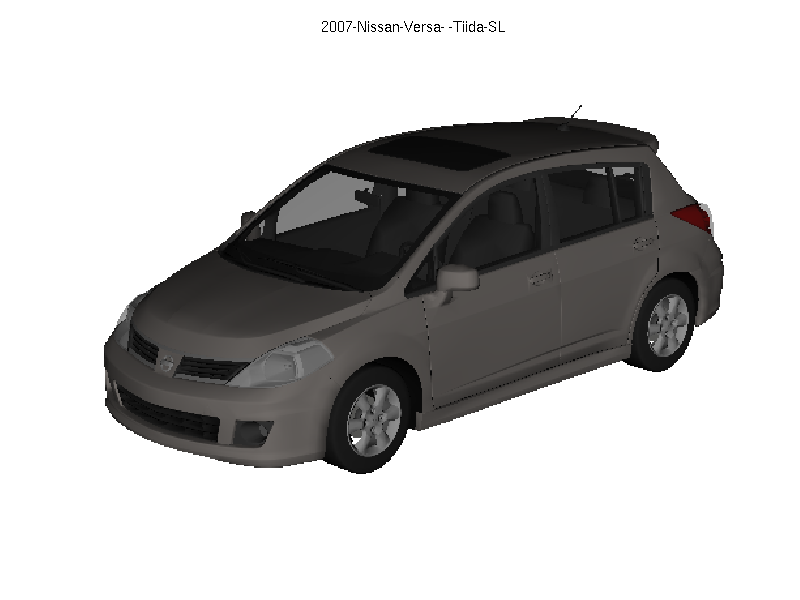
\includegraphics[width=0.16\linewidth]{cad_car/2007-Nissan-Versa-_-Tiida-SL} & 
  %  %       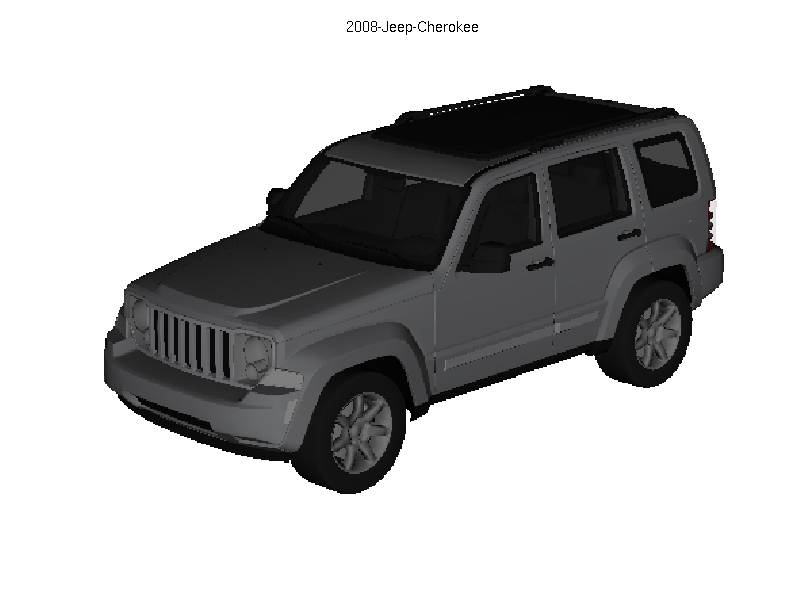
\includegraphics[width=0.16\linewidth]{cad_car/2008-Jeep-Cherokee} \\ 
  %  %       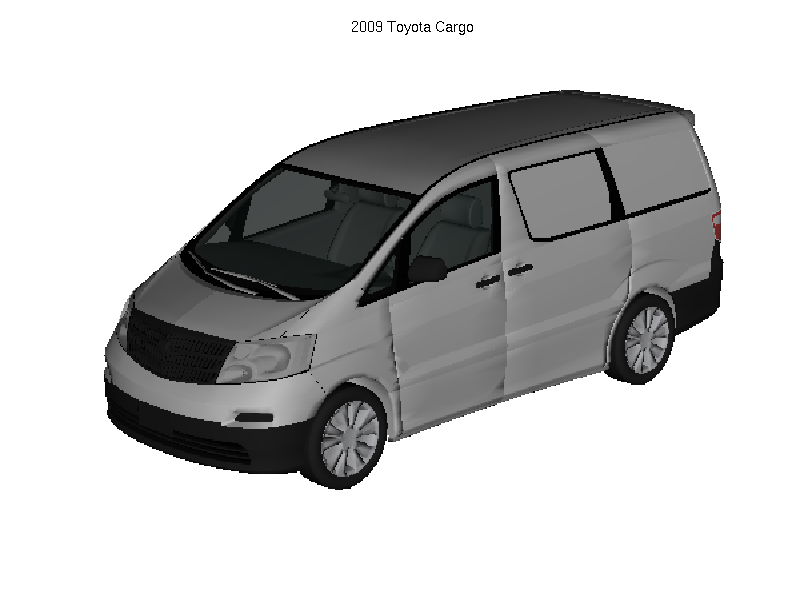
\includegraphics[width=0.16\linewidth]{cad_car/2009 Toyota Cargo} & 
  %  %       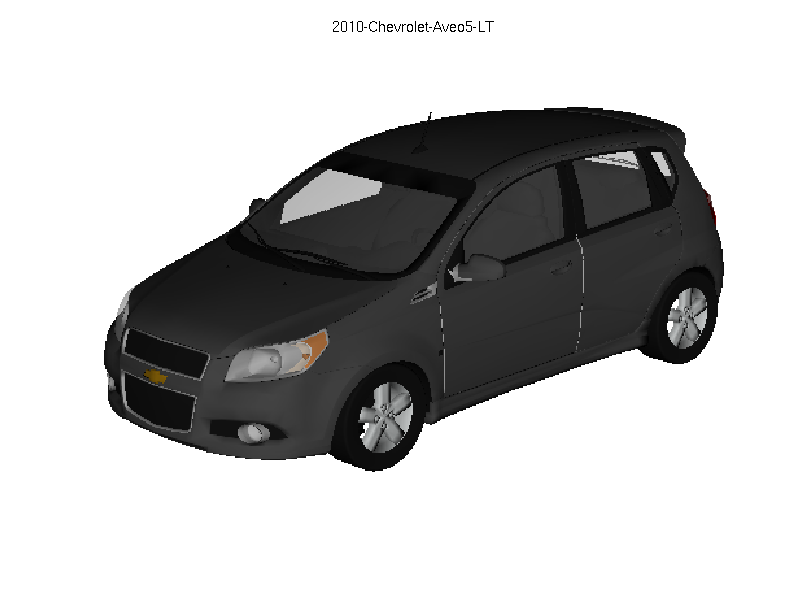
\includegraphics[width=0.16\linewidth]{cad_car/2010-Chevrolet-Aveo5-LT} \\ 
  %  %       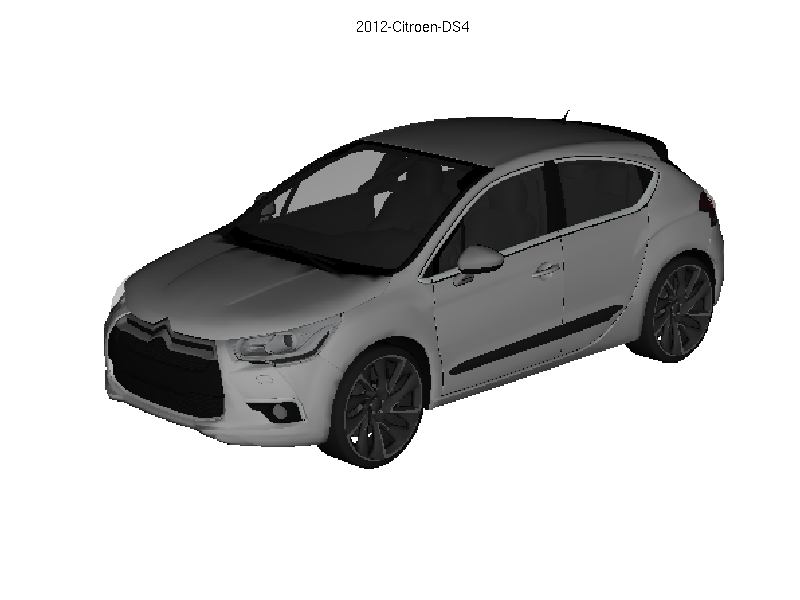
\includegraphics[width=0.16\linewidth]{cad_car/2012-Citroen-DS4}  
  %  %   \end{tabular}
  % \end{tabular}\\
  % (b)
  \caption{Using a bank of CAD models, we generate NZ-WHO templates which can be used to either detect objects directly or initialize pose of an object in the bounding box from other detectors. Once initialization is given, we use NZ-WHO to propose and validate plausible pose on-the-fly and further tune the translation, 3D viewpoint and focal length continuously.}
  % \vspace{-1em}
  \label{fig:front}
\end{figure}
 
% Object detection task has long been about predicting rectangular bounding boxes around the object. In this workthere has been significant many powerful object detectors such as Convolutional Neural Network or Part-Based Models \cite{Girshick14, Felzenszwalb10, Pepik12} 

Current approaches to object class detection have reached a remarkable
level of performance in 2D bounding box
localization~\cite{pascal12,Felzenszwalb10,Girshick14}, due to their
ability to generalize across differences in object appearance,
lighting, and viewpoint. While this generalization
ability of these methods is benefitial for robustness, it also limits
the level of detail that these detectors can deliver as an output.

As a consequence, there has been increased interest in multi-view object
recognition, where viewpoint estimates are provided by
detectors in addition to 2D bounding boxes. Several attempts have been
made to estimate viewpoint along with object class detections,
implemented as extensions to existing detectors, such as the implicit
shape models~\cite{}, the constellation model~\cite{}, or the
deformable part model~\cite{Xiang12,Pepik12,Fidler12,Hejrati14}.

Recently, an even higher level of geometric detail was reached in the
form of aligning
3D CAD model instances to real world test images~\cite{Aubry14,
  Lim14,Kholgade14, Chen13, Kostas14}. Interestingly, the problem of matching 3D models to 2D
images has been explored since the early days of computer
vision~\cite{Lowe87}, but had largely been neglected in recent years
in favor of 2D detectors based on robust local features and
statistical learning techniques. Now, this problem is being revisited
mostly due to two reasons: {\em (i)} the availability of 3D CAD models
for many object classes and {\em (ii)} the availability of robust
image matching techniques.
%
% performance object detectors usually generalizes very well. It
% can handle various intraclass variability, viewpoint change and
% occlusion. However due to this high generalization, sometimes it is
% very difficult to get accurate pose, category or 2D-3D matching. Our
% method, specialized in giving such accurate information, can be
% applied on any generic object detectors to give high quality metadata.
% %
% Matching 3D CAD model to an image has been a classical problem that
% dates back to eighties . Lowe \etal , the vision
% community instead focused on the object detection tasks that estimates
% a rectangular bounding box around an object\cite{Felzenszwalb10,
%   Girshick14}. 
%
%In addition, there has been a growing emand for accurate 2D-3D
%matching \cite{Kholgade14, Chen13, Kostas14} for image manipulation,
%editing, and data augmentation in the computer graphics community.
%
% Recently, with the powerful computing capabilities and a large
% collection of CAD models, the 2D-3D matching (registration) problem
% gets more and more approachable but due to inherent difficulty and
% limited performance of existing methods, many applications still
% require supervision to achieve 2D-3D matching.
% In medical community, registering 3D scan data to 2D image enabled various minimally invasive surgeries \cite{Markelj12}.
%
% For category-level matching, \cite{Xiang12, Hejrati14, Pepik12} used
% 3D parts or aspect to represent underlying category-level 3D geometry
% of the object. With the advent of large public CAD datasets
% \cite{Trimble, Yobi}, the instance-level object detection and 2D-3D
% registration became possible. \cite{Aubry14, Lim14} used large
% collection of CAD models to faithfully align 3D CAD model to an image
% by rendering CAD models and creating 2D templates for various
% viewpoints.

For (i), recent approaches to 2D-3D matching~\cite{Aubry14, Lim14}
typically rely on a
collection of 3D exemplar models, which they render from a
large number of viewpoints. The resulting artifial images are then
used to train exemplar models that can be matched to a real-world
image at test time.
%
For (ii), it has been realized that template-based exemplar detectors
based on HOG~\cite{Dalal05} features can be trained analytically, by
replacing the standard SVM with an LDA classifier
(E-LDA)~\cite{Hariharan12}. As a result, it is feasible to train
hundreds of thousands of mid-level patch detectors for
recognition~\cite{Aubry14}.
%
Unfortunately, the performance of E-LDA relies crucially on an
additional calibration step that equalizes the detection scores of
independently trained exemplar models. Since this step involves costly
mining of hard negative examples~\cite{Dalal05,Felzenszwalb10} on a
validation set, it constitutes the major computational bottleneck of
E-LDA, limiting its scalability.

In this paper, we propose a novel method for 2D-3D alignment of
exemplar CAD models to real-world images that circumvents the need for
calibration, and greatly enhances the scalability of E-LDA. As a
result, we can render novel views and train corresponding exemplar
models {\em on the fly}, without the need for offline processing. As a
by-product, we can formulate the alignment problem as a parameter
search in a continuous pose space, consisting of yaw, pitch and roll, resulting in truely continuous pose estimates, which
we implement using MCMC sampling.
%  require a large number of rendering and 2D
% templates for each of the CAD model with specific viewpoint. Since
% there are so many templates that it becomes almost impossible to get
% all the true positive image from training data. Instead \cite{Aubry14,
%   Lim14} used whitening as a preprocessing stage \cite{Hariharan12} to
% make templates more discriminative. Then calibration is done on a
% small training dataset.
%
% Although whitening to create template is faster than some of
% instance-level matching algorithms such as training Exemplar-SVM
% \cite{Malisiewicz11} or complicated models such as LEVAN
% \cite{Divvala14}, whitening and calibration large number of templates
% takes very long time. Also, once the fixed discrete viewpoint
% templates have been made and calibrated, it is difficult to fine-tune
% the prediction made using the large collection of templates.

Our paper makes the following specific contributions.

First, we present a novel method for training exemplar models from
rendered 3D CAD data {\em on the fly}, enabled by a novel variant of
E-LDA, and making efficient use of the specific characteristics of
rendered images. To our knowledge, our method constitutes the first
attempt to simultaneously render and train exemplar detectors on the
fly.
% In our paper, we present Non-Zero Whiten Histograms of Orientations
% (NZ-WHO) to dramatically speed up the template generation and get rid
% of time consuming calibration and yet achieves performance on par with
% calibrated templates. First, we will present NZ-WHO is more
% discriminative than WHO and introduce Conjugate Gradient method to
% speed up the whitening and create a high resolution template in just
% 80 milliseconds. Also, using this fast NZ-WHO template generation, we
% present \textbf{on-the-fly} template generation to fine tune an
% initial pose estimation to continuously refine translation, viewpoints
% (yaw, roll, pitch) and focal length.

Second, we show to enrich the output of an existing object class
detector, such as the DPM~\cite{Felzenszwalb10} or the
R-CNN~\cite{Girshick14} with additional 3D information, applying our
method to candidate detections provided by the respective detector. As
a result, we can refine the original detections with additional
estimates of 3D continuous pose and a 3D CAD model exemplar.

And third, we give an in-depth experimental study that demonstrates
the effectiveness of our approach on a standard benchmark for
object detection and viewpoint estimation~\cite{Xiang14}. 

\begin{comment}
\scream{Are we keeping the paragraphs from here...}

outperforming previous results on this dataset by considerable
margins.



%% Our contribution
With this growing usage of WHO template and Computer Graphics
rendering, we decided to analyze WHO feature
[Find More Usage of WHO and CG rendering \cite{Pepik12}]




Our pipeline is simple, fast only requires CAD models and no
validation images for calibration. This can be used for post
processing stage of generic object detection. Our pipeline requires
only few minutes to make templates for rough viewpoints and 


We propose a simple method to register the most similar CAD model to
an image and fine-tune viewpoint continuously without discriminative
part search, training nor calibration. Our method is simple, fast and
light-weight in terms of memory so that it can be easily applied on
top of generic object detectors as a final stage of detection or can
be used as a standalone detector. 



% Although our method is geared toward instance-level 2D-3D matching, we evaluated the performance of the templates on PASCAL 2007 and PASCAL 2012 and PASCAL 3D dataset to measure the performance. 

Our tuning stage not only refine position, scale and viewpoint, but
also focal length as well to literally "fine-tune" the initial
proposal. Though our 2D-3D matching method can be used as a
rudimentary object detector, our simple tuning stage can be applied to
any generic object detector to achieve state-of-the-art viewpoint
estimation method.


Finally, we show several applications using our method. Since we have
metadata such as CAD model and geometry, we reconstruct the object
using 2D-3D matching. Also, since we do not need training image, we
show that our 2D-3D matching performs better than standard detectors
in categories where training data is insufficient. We then use our method for
image query to pull out the closest CAD model in a bank of CAD models.


Finally, unlike several CAD model alignment methods that uses  WHO
\cite{Aubry13, Aubry14, Lim14}, we propose a novel pipeline that does
not require calibration which is infeasible in continuous viewpoint
estimation. We propose a simple add-on stage that can enrich object
detections with high-quality 2D-3D alignment. The pipeline is simple
and light weight so this can be easily adapted to be used for any
generic object detectors. Also to facilitate future work, all our
alignment result on PASCAL12 and code are publicly available online.




% Recently, matching a 3D CAD model to an image, 2D-3D matching (registration), is gaining great momentum in various fields of study. 2D-3D matching using Structure from Motion \cite{Sattler11} uses existing 3D model to match the model to a query image. Also image manipulation using 3D CAD models has proven its potential. Kholgade \etal \cite{Kholgade14} and Chen \etal \cite{Chen13} require human input to match 3D models to an image to created realistic morphing or manipulation of the registered object. However, all these application requies human input. In this paper, we propose a novel on-the-fly template generation algorithm that can generate template quickly and validate 2D-3D pose and focal length continuously.

% Our code has been made publicly online \cite{Choy14} so that our algorithm can be used as a pipeline for 2D-3D registration after general purpose object detectors.

\scream{... to here?}
\end{comment}




